\chapter{Metodología}
\section{Levantamiento de información}
El departamento de ingeniería mecánica en el Campus Casa Central, posee una máquina de fatiga (MF) uniaxial en flexión en el laboratorio de tecnología de materiales. \textcolor{red}{Revisar nombre del lab} que se encuentra en la universidad hace más de 50 años, sin saber su fecha exacta de adquisición. La medición de fatiga es realizada a través del método de \textit{esfuerzo-vida}, utilizando la configuración de \textit{rotating bending}, ambos descritos en el capítulo anterior. La información existente sobre la máquina de ensayos es escasa, principalmente por su antigüedad, la perdida de documentos y obsolescencia de la electrónica. Por lo mismo, parte del trabajo de esta memoria se centra en lograr rescatar información y su posterior comprensión para lograr la tener la máquina de fatiga operativa.

\begin{figure}
\centering
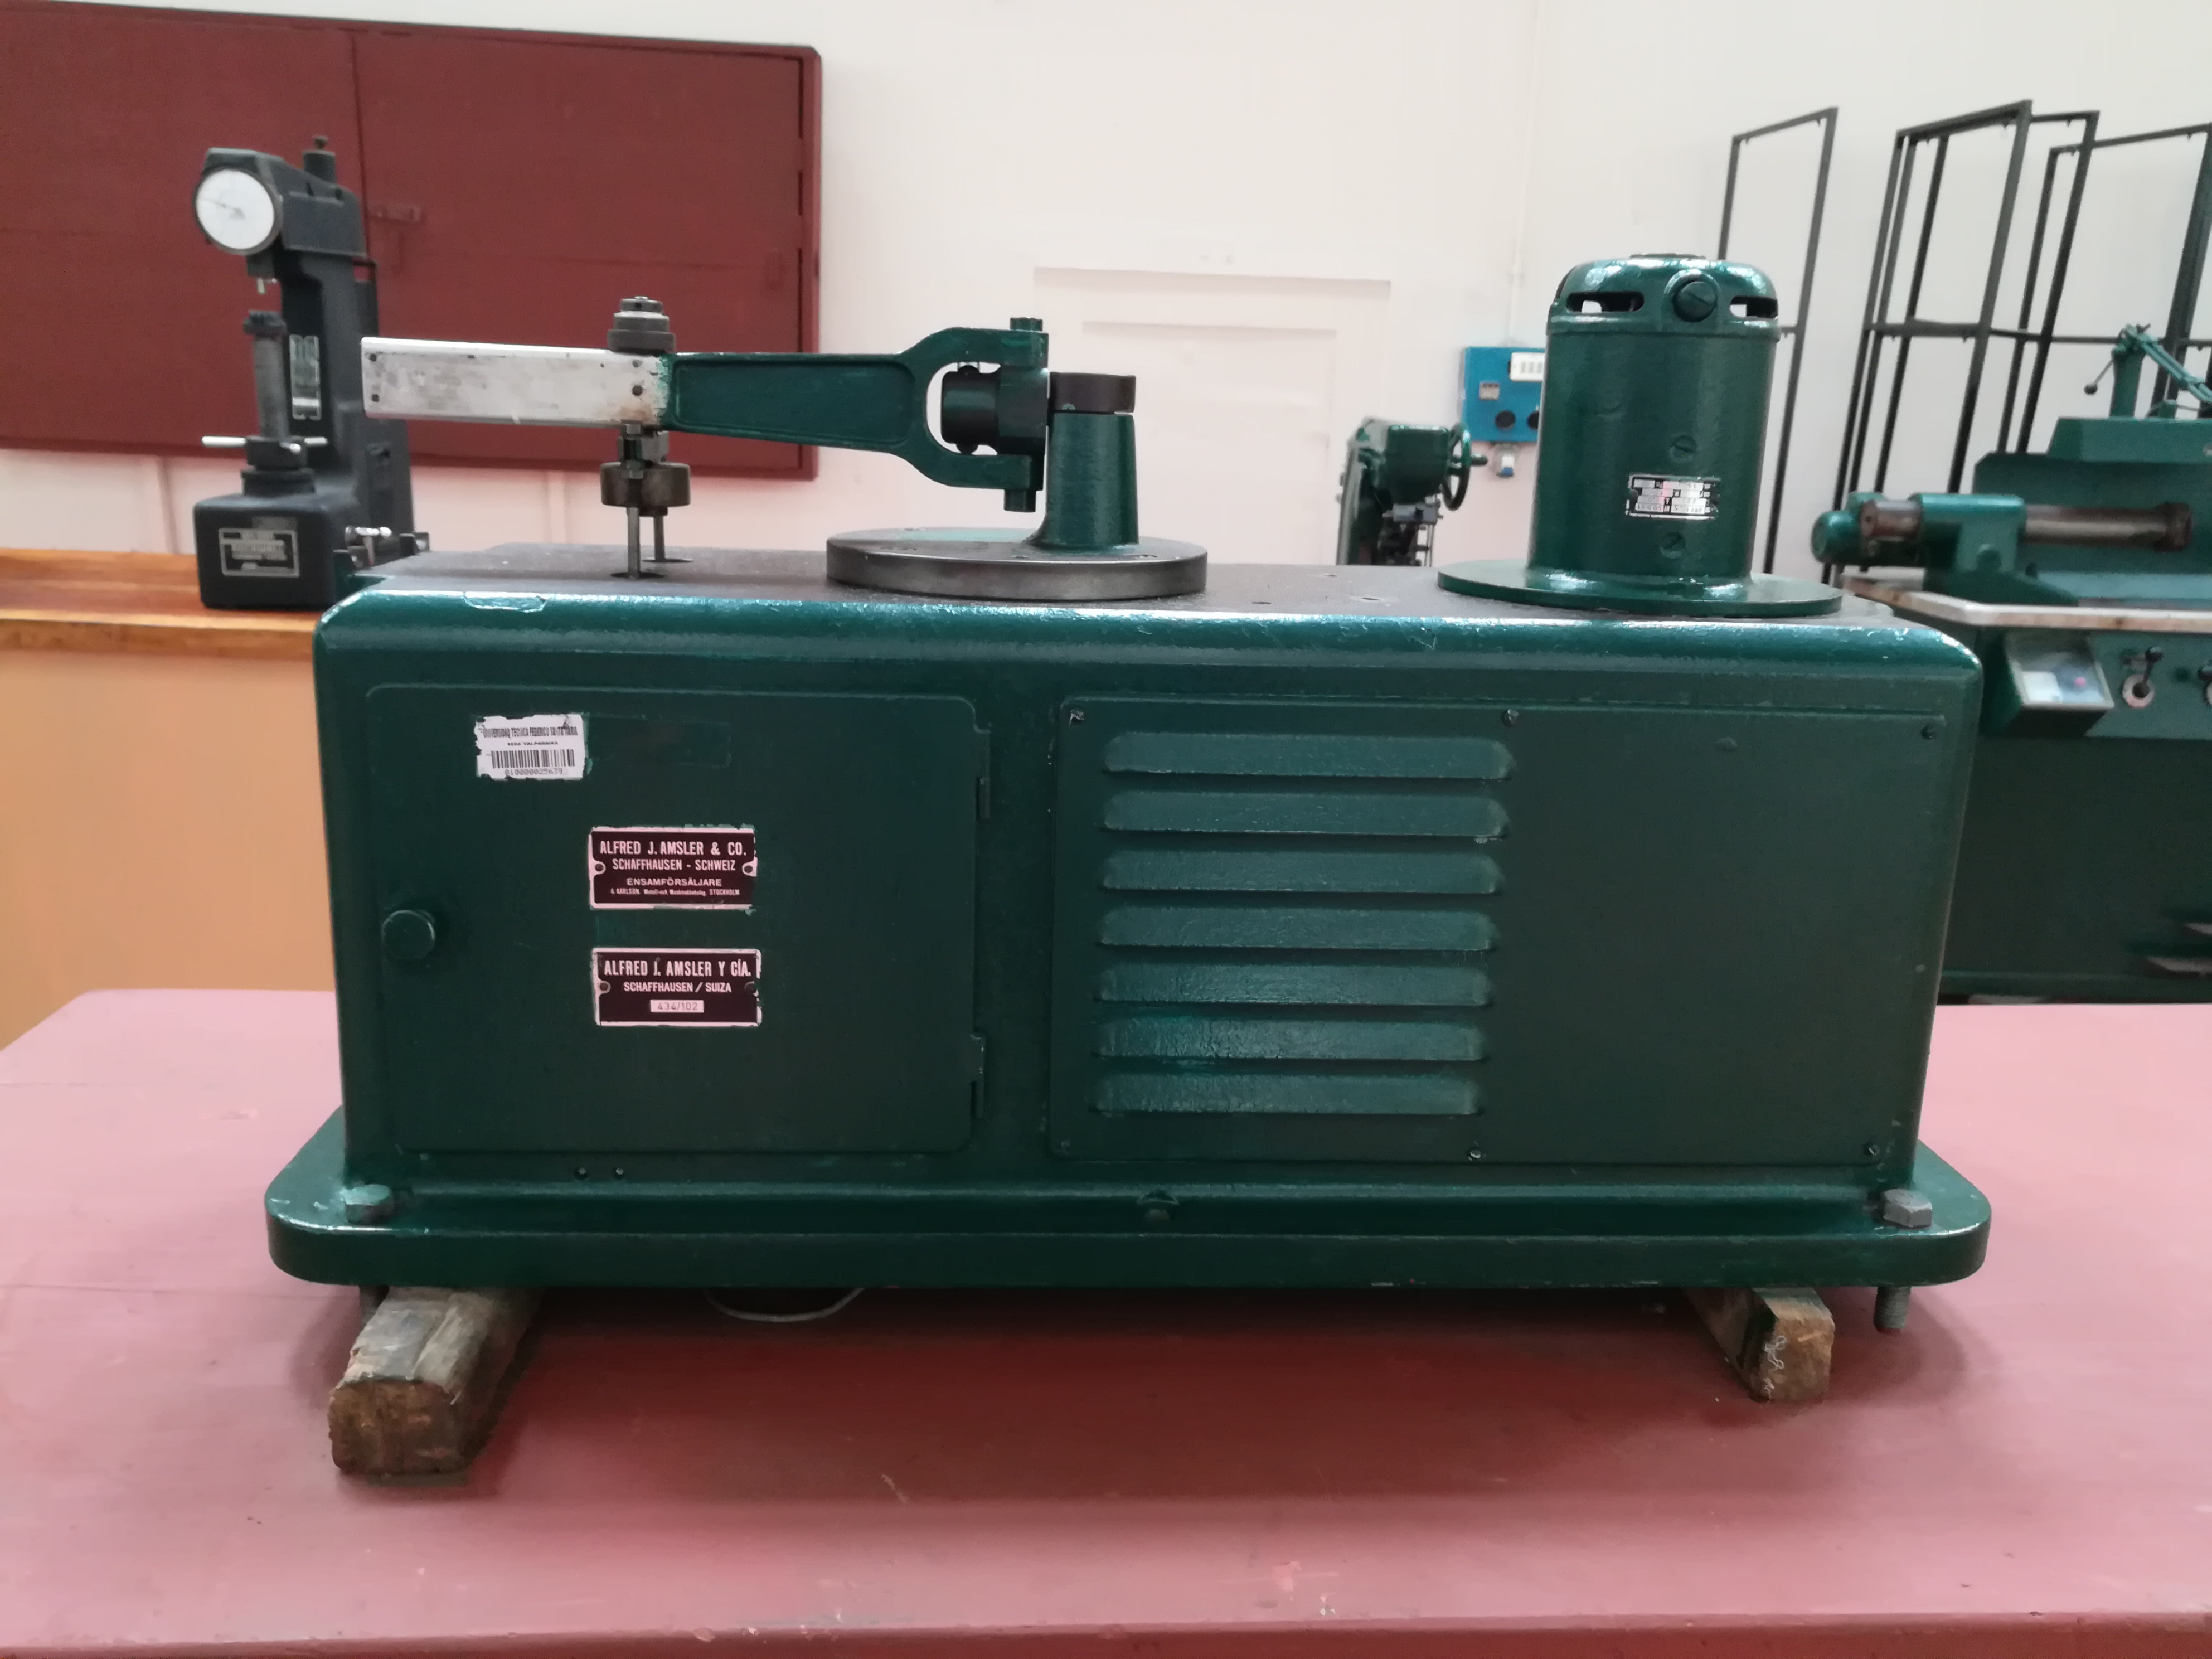
\includegraphics[scale=0.05]{Imagenes/maq_del.jpg}
\label{fig:maq_del}
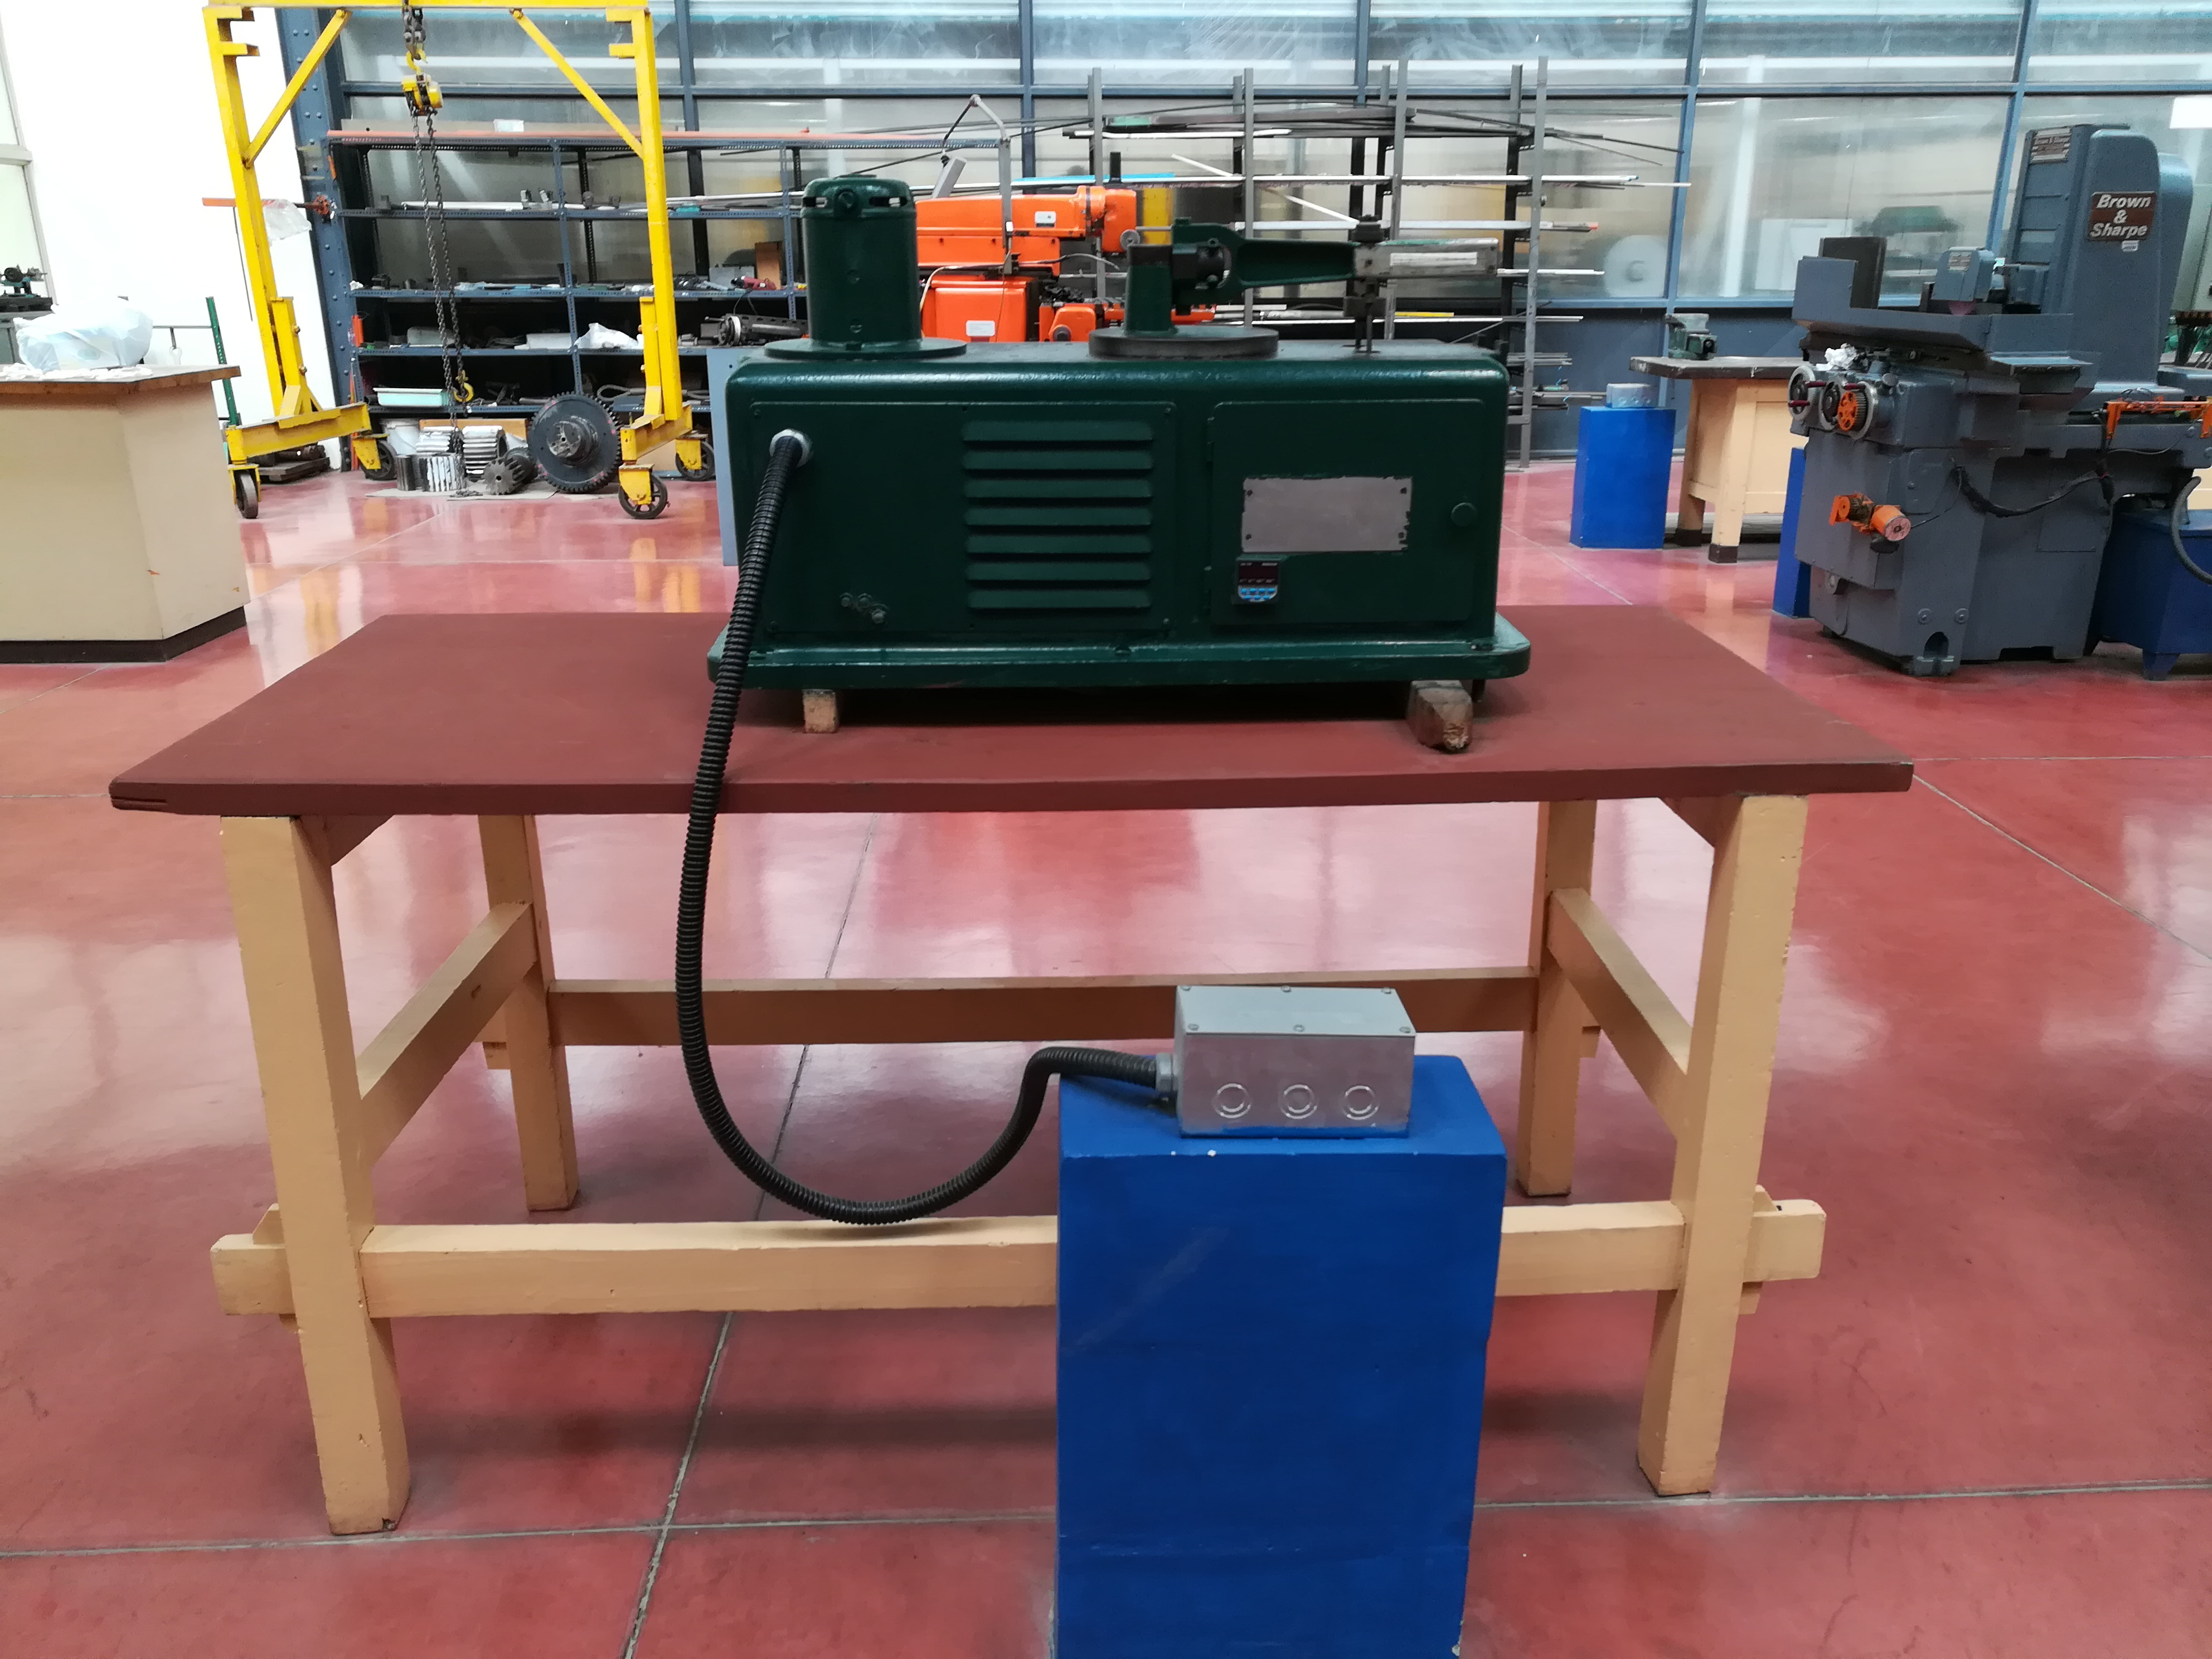
\includegraphics[scale=0.05]{Imagenes/maqfull_post.jpg}
\label{fig:maqfull_post}
\caption{Máquina de fatiga en flexión en el laboratorio de tecnología mecánica}
\label{fig:maq_fat}
\end{figure}


\subsection{Estado actual}
Actualmente la máquina no puede ser utilizada por no estar anclada al piso, estando apoyada sobre dos listones de madera, que a su vez, están sobre una mesa de madera como se aprecia en la figura REF. Por consiguiente, al ser utilizada la máquina comienza a vibrar, saltar y desplazarse lateralmente, lo que impide su uso prolongado por motivos de seguridad. Es decir, no es posible realizar correctamente un ensayo de fatiga de ningún material ni configuración.

La única modificación, según la información recopilada, consiste en el cambio del contador de revoluciones o ciclos realizados en un ensayo de fatiga. Esta actualización consistió en sacar el contador mecánico original y reemplazarlo por un contador electrónico, el cual tiene sus controles y el display adosada a su estructura, como se puede apreciar en la figura \textcolor{red}{agregar imagen del contador}. 

El sistema eléctrico de la máquina permanece intacto, la cual se encuentra conectada a la red de la universidad. Conserva su motor eléctrico original \textcolor{red}{averiguar que tipo de motor es}, junto a un sistema cuya función es suministrar energía de manera continua y estable al motor, para evitar que el ensayo de fatiga se pueda ver afectado por problemas y las variaciones del suministro eléctrico. El motor es de \textcolor{red}{corriente continua} con velocidad constante y sus especificaciones se pueden ver en la tabla \ref{tab:motor_maq} :
\begin{table}[h]
\centering
\begin{tabular}{ll}
\hline
Especificaciones Motor                            & \multicolumn{1}{l}{}    \\ \hline
Tensión                                           & 220 {[}V{]}        		\\
Corriente                                         & 0,8 {[}A{]}        		\\
Factor de potencia (\textbackslash{}cos $\varphi$ & Sin información    		\\
Potencia                                          & 100 {[}W{]}        		\\
Velocidad                                         & 1500 {[}rev/min{]} 		\\ \hline
\end{tabular}
\caption{Especificaciones del motor de la máquina de fatiga.}
\label{tab:motor_maq}
\end{table}

Otro elemento distinto al original consiste en la correa de transmisión entre el motor eléctrico y el disco desbalanceado. La original consistía en una correa de cuero plana y cruzada, sin información respecto a su empalme. La correa actual consiste también en una correa plana y cruzada, sin embargo, su material es tela y el empalme es realizado a mano con hilo acerado. Cabe destacar que lo poco usual de las dimensiones, características y la necesidad de hacer el empalme en la misma máquina, dificulta la búsqueda de una correa que pueda cumplir de manera óptima la transmisión de potencia. Parte de estas dificultades se deben a que el sistema de transmisión no ha sido modificado donde sus poleas tienen dimensiones, tanto de diámetro como de ancho, que no están normalizadas o se encuentran fuera de catálogo de mucho proveedores. 

Por otro lado, los elementos de agarre de la probeta no tienen modificaciones conocidas, tanto el brazo que recibe el movimiento como el agarre empotrado a la estructura de la máquina. La fabricación de las probetas utilizadas se realiza en el mismo laboratorio a partir de acero AISI 1020 o 1040, el cual para conseguir las dimensiones de la figura REF. se debe cortar y tornear.

Finalmente, para realizar los ensayos en distintas configuraciones existen distintas masas (figura REF) que desequilibran el disco rotativo, como se verá en la sección \ref{sec:funcionamiento}, y estas combinaciones se especifican en una tabla de cargas (Anexo REF). Sin embargo, se desconoce el origen, y en consecuencia, la fiabilidad de la información contenida en esta tabla.

\subsection{Funcionamiento}
\label{sec:funcionamiento}
La máquina de fatiga tiene como objetivo lograr que para cada ciclo se ejerza el mismo esfuerzo determinado sobre la probeta, en forma de flexión. Para lograr esto, el mecanismo utilizado es un disco desequilibrado girando a una velocidad constante $\dot{\theta}$, la fuerza es transmitida hasta un brazo que sostiene a su vez a la probeta, generando flexión en la probeta con un doble empotramiento. La velocidad $\dot{\theta}$ del disco se transmitida desde el motor eléctrico a través de poleas y una correa de transmisión en una relación de 1:1 \textcolor{red}{revisar}, a una velocidad de 1500 revoluciones por minuto. Así, para realizar las mediciones de fatiga a distintas cargas se modifica el desequilibrio del disco a través de un conjunto de masas, mostradas en la figura REFcolocarimagenmasas, que permiten generar distintas configuraciones y, por consiguiente, esfuerzos en la probeta. 

Los elementos utilizados para desbalancear son 6 discos pequeños de X \textcolor{red}{medir radio masas} a Y de diámetro. Estos son enumerados del 1 al 5, donde el 1 es el más liviano y el 5 el más pesado, todos de distinto peso a excepción del quinto que se encuentra repetido. Estas se colocan en los extremos del disco giratorio, como se ve en la figura REFimagendisco, dependiendo de la carga que se desee generar. Para conocer que configuración corresponde a cada esfuerzo aplicado sobre la probeta, se utiliza la tabla de cargas señalada anteriormente.

Esta tabla, con 3 columnas de información como se ve en el Anexo REF, nos entrega el esfuerzo normal $\sigma$, el cortante $\tau$ y la combinación necesaria para generar esos esfuerzos. Los números entre paréntesis nos indican cuantas masas se deben apilar en cada perno adosado al disco giratorio, los cuales llamaremos puntos de desequilibrio (PE). Así, la tabla nos señala que la fuerza es producto de la diferencia de masa entre cada PE o la suma de las masas de cada paréntesis. A modo de ejemplo, en la tabla \ref{tab:ejemplo_config} se han colocado las 4 primeras filas de la tabla de cargas, añadiendo 4 columnas con información adicional. En las columnas $m_1$ y $m_2$ se aprecia la suma de cada masa colocada en sus puntos de desequilibrio señalado por la columna de ``Combinación''. La columna $\Delta m$ muestra la diferencia $(m_1-m_2)$ y $m_{total}$ la suma $(m_1+m_2)$. 

\begin{table}[h]
\centering
\label{tab:ejemplo_config}
\begin{tabular}{@{}cclllll@{}}
\toprule
$\sigma \left[\frac{\text{kg}_f}{\text{cm}^2}\right]$ & {$\tau \left[\frac{\text{kg}_f}{\text{cm}^2}\right]$} & Combinación     & $m_1$ {[}g{]} & $m_2$ {[}g{]} & $\Delta m$ {[}g{]} & $m_{total}$ {[}g{]} \\ \midrule
40                                                   & 20                                                                    & (5) - (1+2+3+4) & 30,9199       & 30,5071       & 0,4128             & 61,427              \\
80                                                   & 40                                                                    & (1) - (0)       & 0,7582        & 0             & 0,7582             & 0,7582              \\
120                                                  & 60                                                                    & (5) - (4+2+3)   & 30,9199       & 29,7489       & 1,171              & 60,6688             \\
160                                                  & 80                                                                    & (2) - (1)       & 2,2969        & 0,7582        & 1,5387             & 3,0551              \\ \bottomrule
\end{tabular}
\caption{Tabla de configuración de las masas modificada, mostrando el peso, su diferencia y el total para cada combinación}
\end{table}

%\subsubsection{Mecánica}
%\subsubsection{Electrónica}
%\subsubsection{Recolección de datos}
\subsection{Mediciones}

\section{Diseño de estructura}
\subsection{Diseño en soporte de acero}

\subsection{Diseño en madera}

\subsection{Cálculo de cargas en estructura de madera}

\subsection{Uniones}
\subsubsection{Acero - madera}
\subsubsection{Madera - Madera}
\subparagraph{Pernos}
\subparagraph{Tirafondos}
\subsubsection{Herrajes y conectores}

\subsection{Simulaciones}
\subsubsection{Estática}
\subsubsection{Modal}


\section{Modelo del sistema de funcionamiento}
\subsection{Diagrama del sistema}

\subsection{Modelo del sistema}
\subsubsection{Simplificaciones}
\subsubsection{Modelo del disco desbalanceado}
\subsubsection{Cálculo y obtención de valores del sistema}

\subsection{Ecuaciones de movimiento de la máquina de fatiga}

\subsection{Carga sobre la probeta}

\section{Análisis de información existente}
\subsection{Simulación de cargas}